\cleardoublepage

\chapter{Résultats - Discussions}

Je vais maintenant vous présenter dans ce chapitre la solution obtenue après le développement et la livraison au client.
De plus je présenterai mes impressions durant sa réalisation, dans le domaine technique et fonctionnel.

%%%%%%%%%%%%%%%%%%%%%%%%%%%%%%%%%%%%%%%%%%%%%%%%%%%%%%%%%%%%%%%%%%%%%%%%%%%
%%%%%%%%%%%%%%%%%%%%%%%%%%%%%%%%%%%%%%%%%%%%%%%%%%%%%%%%%%%%%%%%%%%%%%%%%%%
%%%%%%%%%%%%%%%%%%%%%%%%%%%%%%%%%%%%%%%%%%%%%%%%%%%%%%%%%%%%%%%%%%%%%%%%%%%
%%%%%%%%%%%%%%%%%%%%%%%%%%%%%%%%%%%%%%%%%%%%%%%%%%%%%%%%%%%%%%%%%%%%%%%%%%%
%%%%%%%%%%%%%%%%%%%%%%%%%%%%%%%%%%%%%%%%%%%%%%%%%%%%%%%%%%%%%%%%%%%%%%%%%%%

\section{Interface graphique utilisateur}

J'ai été libre de programmer la première version de l'interface graphique, comportant les fonctionnalités demandées par le client.
Ce dernier a tout de même participé à sa réalisation en effectuant diverses critiques et demandes de réagencement des éléments amenant à une interface graphique optimale et ergonomique.

Je présenterai dans cette section la structure de l'affichage et les différents types d'écran de la solution.

%%%%%%%%%%%%%%%%%%%%%%%%%%%%%%%%%%%%%%%%%%%%%%%%%%%%%%%%%%%%%%%%%%%%%%%%%%%
%%%%%%%%%%%%%%%%%%%%%%%%%%%%%%%%%%%%%%%%%%%%%%%%%%%%%%%%%%%%%%%%%%%%%%%%%%%
%%%%%%%%%%%%%%%%%%%%%%%%%%%%%%%%%%%%%%%%%%%%%%%%%%%%%%%%%%%%%%%%%%%%%%%%%%%

\subsection{Connexion}

L'application restreint son accès aux personnes autorisées, c'est à dire possédant des identifiants valides.
Lorsque l'on se connecte à l'application, la première fenêtre qui s'affiche est l'écran de connexion, que l'on peut apercevoir sur la capture d'écran de la figure \ref{connexion_ecran}.
\begin{figure}[!h]
	\center
	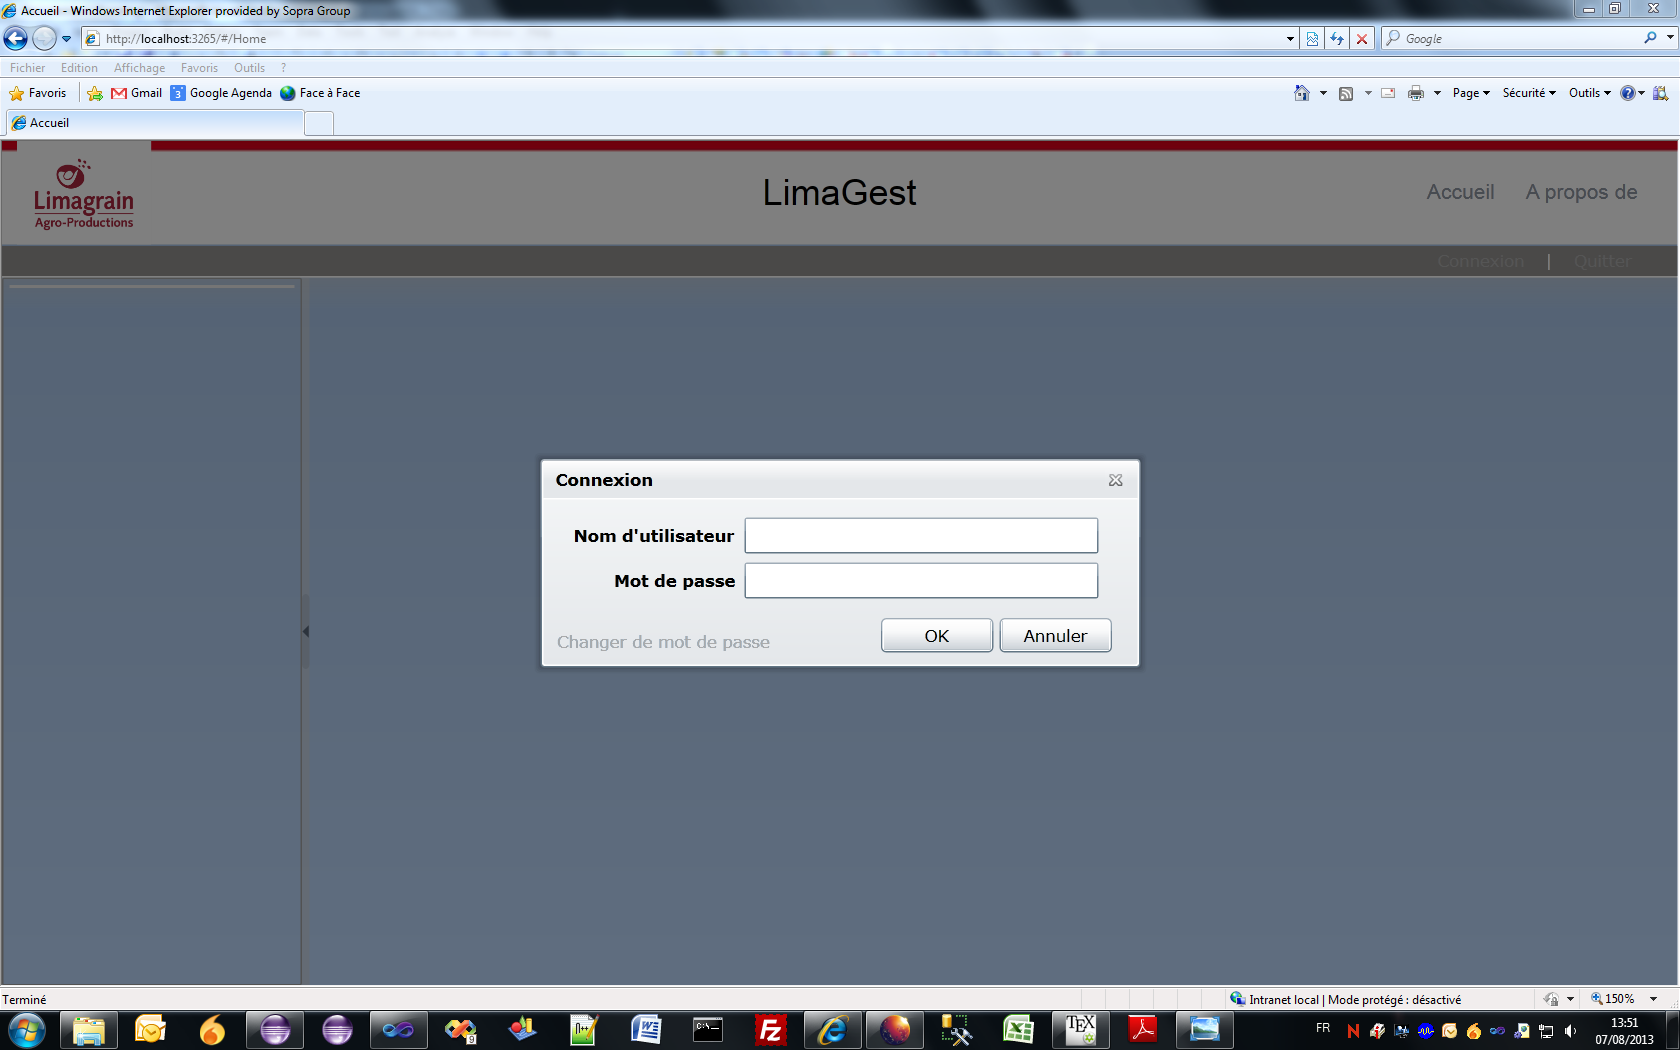
\includegraphics[width=1\textwidth]{img/connexion_ecran.png}
	\caption{Écran de connexion}
	\label{connexion_ecran}
\end{figure}
~~\\

L'application peut se connecter à un serveur LDAP permettant la gestion des utilisateurs.
Lorsque l'utilisateur a saisi son identifiant et son mot de passe, l'application vérifie d'abord s'il s'agit d'un compte LDAP en envoyant une requête au serveur LDAP.
Si ce n'est pas le cas, alors l'application va vérifier s'il s'agit d'un compte "applicatif pur" propre à l'application.
Ce processus est schématisé par le diagramme de flux présent sur la figure \ref{connexion_processus}.
\begin{figure}[!h]
	\center
	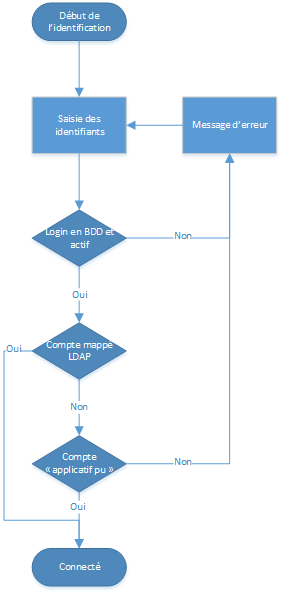
\includegraphics[width=0.4\textwidth]{img/connexion_processus.png}
	\caption{Processus de connexion}
	\label{connexion_processus}
\end{figure}

%%%%%%%%%%%%%%%%%%%%%%%%%%%%%%%%%%%%%%%%%%%%%%%%%%%%%%%%%%%%%%%%%%%%%%%%%%%
%%%%%%%%%%%%%%%%%%%%%%%%%%%%%%%%%%%%%%%%%%%%%%%%%%%%%%%%%%%%%%%%%%%%%%%%%%%
%%%%%%%%%%%%%%%%%%%%%%%%%%%%%%%%%%%%%%%%%%%%%%%%%%%%%%%%%%%%%%%%%%%%%%%%%%%

\subsection{Structure}

La figure \ref{structure} montre la structure de l'interface graphique, avec les trois parties principales : la barre supérieure, le menu latéral, et le contenu où s'affichent les fenêtres.
\begin{figure}[!h]
	\center
	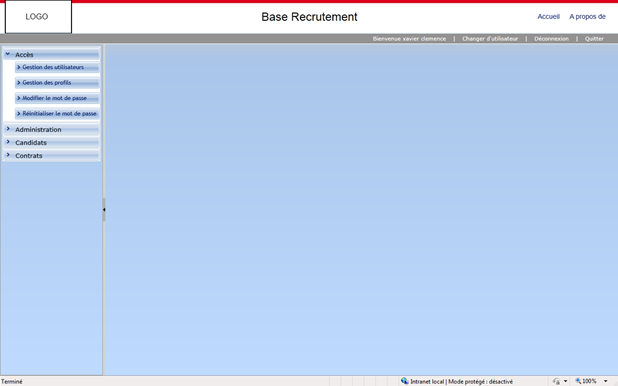
\includegraphics[width=1\textwidth]{img/structure.png}
	\caption{Structure de l'interface graphique}
	\label{structure}
\end{figure}

%%%%%%%%%%%%%%%%%%%%%%%%%%%%%%%%%%%%%%%%%%%%%%%%%%%%%%%%%%%%%%%%%%%%%%%%%%%

\subsubsection{Barre supérieure}

La partie supérieure de l'écran possèdes deux fonctions.
La première est l'affichage des détails de l'application, tels que le logo de l'entreprise, le nom de l'application, et des liens généraux.
Cela permet d'identifier l'application utilisée.
La seconde est liée au compte de l'utilisateur, avec des liens permettant de changer d'utilisateur, de se déconnecter, et permettant de quitter l'application.

%%%%%%%%%%%%%%%%%%%%%%%%%%%%%%%%%%%%%%%%%%%%%%%%%%%%%%%%%%%%%%%%%%%%%%%%%%%

\subsubsection{Menu latéral}

Une barre latérale située sur la partie gauche propose un \textit{menu}.
Chaque ligne de ce menu correspond à un module de l'application, comme expliqué précédemment.
La figure \ref{menu} est une capture d'écran du menu, montrant les différents menus de l'application.

De plus, un sous-menu de second niveau apparait lorsque l'on sélectionne un menu.
Il s'agit de chacun des écrans principaux du module correspondant.
Par exemple, le menu "Accès" possède quatre sous-menus correspondants à quatre fonctionnalités, comme le montre la capture d'écran de la figure \ref{menu}.

\begin{figure}[!h]
	\center
	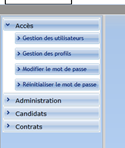
\includegraphics[width=0.5\textwidth]{img/menu.png}
	\caption{Menu latéral gauche}
	\label{menu}
\end{figure}
~~\\

Ce menu facilite la navigation entre les différentes fonctionnalités de l'application sans avoir à retourner sur la page d'accueil.
Les sous-menus quant à eux permettent de hiérarchiser les fonctionnalités par thème, séparant ainsi les actions liées aux candidats de celles liées aux contrats et encore de l'administration.

%%%%%%%%%%%%%%%%%%%%%%%%%%%%%%%%%%%%%%%%%%%%%%%%%%%%%%%%%%%%%%%%%%%%%%%%%%%
%%%%%%%%%%%%%%%%%%%%%%%%%%%%%%%%%%%%%%%%%%%%%%%%%%%%%%%%%%%%%%%%%%%%%%%%%%%
%%%%%%%%%%%%%%%%%%%%%%%%%%%%%%%%%%%%%%%%%%%%%%%%%%%%%%%%%%%%%%%%%%%%%%%%%%%

\subsection{Les types d'écran}

Pour ne pas perdre l'utilisateur, deux types d'écrans ont été utilisés, permettant de garder le même style dans l'application.

Un écran d'affichage de données comporte un tableau permettant d'afficher une liste de valeurs.
Il y a une zone de recherche permettant de filtrer les données.
De plus, des boutons situés en bas de l'écran permettent d'effectuer des actions sur le ou les élément(s) sélectionné(s) : affichage des détails, modification, suppression, \ldots

L'affichage, la modification ou la création d'un élément est une fenêtre s'affichant par-dessus l'écran actuel sous la forme d'un pop-up.
Lorsqu'il s'agit d'une édition les éléments sont des "zones de texte" ou des "listes déroulantes", sinon ce sont simplement des "labels".

Deux écrans de "paramétrage" sont différents des autres.
Ils permettent de gérer les tables "statiques" contenant les valeurs des différentes listes déroulantes que l'on peut trouver dans l'application.
Ils sont composés de plusieurs tableaux affichant les données présentes, avec des boutons permettant l'ajout, la modification ou la suppression de valeurs.

%%%%%%%%%%%%%%%%%%%%%%%%%%%%%%%%%%%%%%%%%%%%%%%%%%%%%%%%%%%%%%%%%%%%%%%%%%%
%%%%%%%%%%%%%%%%%%%%%%%%%%%%%%%%%%%%%%%%%%%%%%%%%%%%%%%%%%%%%%%%%%%%%%%%%%%
%%%%%%%%%%%%%%%%%%%%%%%%%%%%%%%%%%%%%%%%%%%%%%%%%%%%%%%%%%%%%%%%%%%%%%%%%%%
%%%%%%%%%%%%%%%%%%%%%%%%%%%%%%%%%%%%%%%%%%%%%%%%%%%%%%%%%%%%%%%%%%%%%%%%%%%
%%%%%%%%%%%%%%%%%%%%%%%%%%%%%%%%%%%%%%%%%%%%%%%%%%%%%%%%%%%%%%%%%%%%%%%%%%%

\section{Base de données}

%%%%%%%%%%%%%%%%%%%%%%%%%%%%%%%%%%%%%%%%%%%%%%%%%%%%%%%%%%%%%%%%%%%%%%%%%%%
%%%%%%%%%%%%%%%%%%%%%%%%%%%%%%%%%%%%%%%%%%%%%%%%%%%%%%%%%%%%%%%%%%%%%%%%%%%
%%%%%%%%%%%%%%%%%%%%%%%%%%%%%%%%%%%%%%%%%%%%%%%%%%%%%%%%%%%%%%%%%%%%%%%%%%%

\subsection{Modèle de données}

Le modèle de données actuel satisfait bien le besoin du client.
Il représente correctement les différentes données à enregistrer, avec les contraintes et dépendances imposées.

Cependant il reste quelques améliorations possibles.
En effet, le client a tendance à ajouter, modifier ou supprimer certaines spécifications au court du projet, imposant des changes plus ou moins importants dans le modèle.
Ces changements impactent aussi les différentes couches de l'application, du mapping à l'interface graphique, ce qui peut faire perdre un temps important en fin de projet.
Pour ne pas retarder la livraison du lot 1, les modifications "non bloquantes" n'ont pas été apportées et le seront lors du lot 2.

%%%%%%%%%%%%%%%%%%%%%%%%%%%%%%%%%%%%%%%%%%%%%%%%%%%%%%%%%%%%%%%%%%%%%%%%%%%
%%%%%%%%%%%%%%%%%%%%%%%%%%%%%%%%%%%%%%%%%%%%%%%%%%%%%%%%%%%%%%%%%%%%%%%%%%%
%%%%%%%%%%%%%%%%%%%%%%%%%%%%%%%%%%%%%%%%%%%%%%%%%%%%%%%%%%%%%%%%%%%%%%%%%%%

\subsection{Importation des anciennes données}

Plusieurs milliers de candidats et contrats ont été saisis avec l'ancienne application par le service de recrutement.
De nombreux candidats effectuent plusieurs contrats dans le groupe Limagrain.
Pour ne pas avoir à ressaisir ces informations, il est nécessaire d'effectuer une importation des anciennes données dans la nouvelle base de données.
\\

Le changement du modèle de données entre l'ancienne et la nouvelle version de la base de données impose certaines modifications.

Lorsque des champs sont ajoutés et qu'ils sont obligatoires, il est nécessaire de définir leur valeur.
S'il s'agissait d'un simple champs (entier, chaîne de caractères, date, \ldots) alors j'ai soit spécifié la valeur par défaut (0, la chaîne vide, la date minimale, \ldots), soit défini une valeur spécifique que l'utilisateur devra mettre à jour (par exemple "A définir" ou la date du jour), selon ce que modélise le champ.

Si un champ change de type, comme par exemple le passage d'un stockage sous forme de chaîne de caractères (\lstinline{String}) à entier (\lstinline{int}), il est souvent nécessaire d'effectuer une conversion, si cela est possible.
Ce changement de type permet de s'adapter aux besoins de l'utilisateur, ou améliorer la cohérence des données dans la base de données en empêchant le stockage d'informations invalides.

C'était le cas pour un numéro de sécurité social, initialement stocké sous la forme d'une chaîne de caractères, les données seront maintenant stockés sous la forme d'un entier à 15 chiffres.

%%%%%%%%%%%%%%%%%%%%%%%%%%%%%%%%%%%%%%%%%%%%%%%%%%%%%%%%%%%%%%%%%%%%%%%%%%%
%%%%%%%%%%%%%%%%%%%%%%%%%%%%%%%%%%%%%%%%%%%%%%%%%%%%%%%%%%%%%%%%%%%%%%%%%%%
%%%%%%%%%%%%%%%%%%%%%%%%%%%%%%%%%%%%%%%%%%%%%%%%%%%%%%%%%%%%%%%%%%%%%%%%%%%
%%%%%%%%%%%%%%%%%%%%%%%%%%%%%%%%%%%%%%%%%%%%%%%%%%%%%%%%%%%%%%%%%%%%%%%%%%%
%%%%%%%%%%%%%%%%%%%%%%%%%%%%%%%%%%%%%%%%%%%%%%%%%%%%%%%%%%%%%%%%%%%%%%%%%%%

\section{Aspect fonctionnel}

%%%%%%%%%%%%%%%%%%%%%%%%%%%%%%%%%%%%%%%%%%%%%%%%%%%%%%%%%%%%%%%%%%%%%%%%%%%
%%%%%%%%%%%%%%%%%%%%%%%%%%%%%%%%%%%%%%%%%%%%%%%%%%%%%%%%%%%%%%%%%%%%%%%%%%%
%%%%%%%%%%%%%%%%%%%%%%%%%%%%%%%%%%%%%%%%%%%%%%%%%%%%%%%%%%%%%%%%%%%%%%%%%%%

\subsection{Contact avec le client}

Travailler en assistance chez le client m'a permis de découvrir un univers totalement différent de celui de l'agence Sopra Group.

L'avantage est d'être en contact direct avec le client, ce qui permet d'avoir des informations en temps réel. Cela évite donc de devoir appeler ou échanger des mails, et les explications sont plus claires.

En contrepartie, le client a tendance à demander l'état d'avancement du projet plus régulièrement.
Cette proximité procure une pression supplémentaire, notamment lorsque le projet est en retard sur les prévisions.

%%%%%%%%%%%%%%%%%%%%%%%%%%%%%%%%%%%%%%%%%%%%%%%%%%%%%%%%%%%%%%%%%%%%%%%%%%%
%%%%%%%%%%%%%%%%%%%%%%%%%%%%%%%%%%%%%%%%%%%%%%%%%%%%%%%%%%%%%%%%%%%%%%%%%%%
%%%%%%%%%%%%%%%%%%%%%%%%%%%%%%%%%%%%%%%%%%%%%%%%%%%%%%%%%%%%%%%%%%%%%%%%%%%

\subsection{Les spécifications}

Le principal problème rencontré durant ce projet est l'absence de périmètre dans les spécifications.
Celles-ci ont en effet été rédigées en parallèle, voir même en se basant sur les résultats de l'application, par manque de budget et de charges sur le projet.

Cette porte ouverte a permis au client de modifier le périmètre du projet au cours du temps.
De nouvelles fonctionnalités ont été demandées au fur et à mesure de l'avancement.
De plus, certaines fonctionnalités ont dû être modifiées à plusieurs reprises pour répondre aux besoins du client.

%%%%%%%%%%%%%%%%%%%%%%%%%%%%%%%%%%%%%%%%%%%%%%%%%%%%%%%%%%%%%%%%%%%%%%%%%%%
%%%%%%%%%%%%%%%%%%%%%%%%%%%%%%%%%%%%%%%%%%%%%%%%%%%%%%%%%%%%%%%%%%%%%%%%%%%
%%%%%%%%%%%%%%%%%%%%%%%%%%%%%%%%%%%%%%%%%%%%%%%%%%%%%%%%%%%%%%%%%%%%%%%%%%%

\subsection{La communication}

Ce projet m'a amené à utiliser mes compétences de communication à plusieurs reprises et dans diverses situations.
\\

Les besoins de l'utilisateur peuvent parfois prendre un temps important pour être réalisés techniquement.
Il m'est donc arrivé de négocier avec le client pour concevoir une solution intermédiaire, avec le meilleur compromis entre temps de développement et fonctionnalité désirée.
\\

Une fois la première ébauche de l'application terminée, une réunion a été faite chez le client en présence des diverses personnes du service de recrutement qui utiliseront l'application.
Cette réunion avait pour objectif de présenter l'aspect général de l'application, ainsi que les différentes fonctionnalités implémentées.
Il a fallu aussi répondre aux différentes interrogations du client, notamment la date à laquelle sera opérationnelle l'application.